\chapter{Simulation studies}
Suitable search spaces have been selected for the hyperparameters of the various regression methods discussed in Chapter \ref{background}. Hyperparameter tuning has been performed using both approaches discussed in Chapter \ref{tuning} on synthetic datasets generated according to the specification defined in Chapter \ref{sec:datagen}. Various model metrics have been calculated to evaluate the performance of the different regression methods, as well as compare the two parameter tuning approaches.

\section{Simulation setup}
A bundle of 20 synthetic datasets has been generated according to the specification discussed in Chapter \ref{sec:datagen}. Each of the datasets contains 400 observations and is split into a training dataset of 300 and test dataset of 100 observations. Both hyperparameter tuning and fitting of the final models for each approach have been performed on the training dataset. All model metrics have been calculated for the final models on the test dataset.

\section{Hyperparameter search spaces}
Suitable hyperparameter values have been considered in the tuning of the various regression methods. The hyperparameter search spaces for each regression method are shown in Table \ref{tab:tuning_values}. Values for the TTLP and LTLP methods are selected as suggested by \cite{kim2013network}.
{\def\arraystretch{1.5}\tabcolsep=10pt
	\begin{table}[t]
		\label{tab:tuning_values}
		\caption{Hyperparameter search space for all regression methods}
		\centering
		\begin{tabular}{l p{2.8cm} p{6.3cm}}
			\hline\hline 
			Method name & Parameter & Search space \\
			\hline\hline
			Lasso (\ref{sec:lasso})		&Alpha $(\alpha)$&100 values chosen by Scikit-Learn's implementation of the Lasso\\
			\hline
			ENet (\ref{sec:enet})	&Alpha $(\alpha)$&100 values chosen by Scikit-Learn's implementation of the Elastic Net\\
			&L1 ratio&[0.1, 0.25, 0.4, 0.5, 0.6, 0.7, 0.8, 0.9, .95, .99]\\
			\hline
			Grace (\ref{sec:grace})			&Lambda 1 $(\lambda_1)$&[0.01, 0.1, 1, 10, 100, 1000, 10000]\\
			&Lambda 2  $(\lambda_2)$&[0.01, 0.1, 1, 10, 100, 1000, 10000]\\
			\hline
			aGrace (\ref{sec:agrace})		&Lambda 1 $(\lambda_1)$&[0.01, 0.1, 1, 10, 100, 1000, 10000]\\
			&Lambda 2  $(\lambda_2)$&[0.01, 0.1, 1, 10, 100, 1000, 10000]\\
			\hline
			GBLasso (\ref{sec:gblasso})		&Gamma $(\gamma)$&[2, 3, 4]\\
			&Lambda $(\lambda)$&[0.01, 0.1, 1, 10, 100, 1000, 10000]\\
			\hline
			Linf (\ref{sec:linf})			&C&[5, 10, 15, ..., 100]\\
			\hline
			aLinf (\ref{sec:alinf})			&E&[5, 10, 15, ..., 100]\\
			\hline
			TTLP (\ref{sec:ttlp})			&Delta 1 $(\delta_1)$*&3 evenly spaced values in the range $[t,\frac{pt}{4}]$**\\
			&Delta 2 $(\delta_2)$*&3 evenly spaced values in the range $[t,tg]$**\\
			&Tau $(\tau)$&3 evenly spaced values in the range $[10^{-6},\frac{t}{2}]$**\\
			\hline
			LTLP (\ref{sec:ltlp})			&Delta 1 $(\delta_1)$*&3 evenly spaced values in the range $[\frac{\hat{\lambda_{lasso}}}{1.5},1.5\hat{\lambda_{lasso}}]$**\\
			&Delta 2*, Tau&Same as TTLP\\
			\multicolumn{3}{p{13.5cm}}{*Where Lambda 1 $(\lambda_1) = f(\delta_1,\tau) = \frac{\delta_1}{\tau}$ and Lambda 2 $(\lambda_2) = f(\delta_2,\tau) = \frac{\delta_2}{\tau}$}\\
			\multicolumn{3}{p{13.5cm}}{**Where $t$ is the maximum absolute value of the coefficients estimated by the Lasso, $p$ is the number of predictors, $g$ is the number of edges in the network and $\hat{\lambda_{lasso}}$ is the tuning parameter value selected by the Lasso}\\
			\hline
			Composite (\ref{sec:comp_reg})	&Vote Threshold&[0.1, 0.2, 0.3, ... 1]\\
			\hline
		\end{tabular}
	\end{table}
}

\section{Model metrics}
A combination of prediction evaluation and variable selection metrics has been used to compare the regression and hyperparameter tuning methods discussed in the previous chapters.

\subsection{Prediction evaluation metrics}
The mean squared error (MSE) is calculated as defined in Section \ref{sec:trad_tuning} on the independent test datasets. 

\subsection{Variable selection metrics}
Ground truth about the true relationships between the predictors and the target variable is available resulting from the use of synthetic datasets for model selection and evaluation. Knowing the true predictor coefficients, we can define a number of metrics to evaluate the variable selection of each model. Note the use of Iverson bracket notation to express conditional counting in Equations \ref{eq:sensitivity}, \ref{eq:specificity} and \ref{eq:precision}.

\subsubsection{Correlation}
We define the Correlation metric of a model $M$ as the Pearson correlation coefficient between the estimated coefficient vector $\beta_M$ and the true coefficient vector $\beta_{true}$ as shown in Equation \ref{eq:correlation}. 
\begin{equation} \label{eq:correlation}
Correlation(M) = \rho_{\beta_M,\beta_{true}} = \frac{cov(\beta_M,\beta_{true})}{\sigma_{\beta_M} \sigma_{\beta_{true}}}
\end{equation}

\subsubsection{Sensitivity}
We define the variable selection Sensitivity of a model $M$ as the fraction of correctly identified relevant predictors. Formally, this is the fraction of predictors with non-zero coefficients in the true coefficient vector $\beta_{true}$ that correctly have non-zero coefficients in the estimated coefficient vector $\beta_M$ as shown in Equation \ref{eq:sensitivity}. 
\begin{equation} \label{eq:sensitivity}
Sensitivity(M) = \frac{\sum_{i=1}^{p}[\beta_{true_i} \ne 0, \beta_{M_i} \ne 0]}{\sum_{i=1}^{p}[\beta_{true_i} \ne 0]}
\end{equation}

\subsubsection{Specificity}
We define the variable selection Specificity of a model $M$ as the fraction of correctly identified irrelevant predictors. Formally, this is the fraction of predictors with zero coefficients in the true coefficient vector $\beta_{true}$ that correctly have zero coefficients in the estimated coefficient vector $\beta_M$ as shown in Equation \ref{eq:specificity}. 
\begin{equation} \label{eq:specificity}
Specificity(M) = \frac{\sum_{i=1}^{p}[\beta_{true_i} = 0, \beta_{M_i} = 0]}{\sum_{i=1}^{p}[\beta_{true_i} = 0]}
\end{equation}

\subsubsection{Precision}
We define the variable selection Precision of a model $M$ as the fraction of identified predictors that are truly relevant. Formally, this is the fraction of predictors with non-zero coefficients in the estimated coefficient vector $\beta_M$ that have non-zero coefficients in the true coefficient vector $\beta_{true}$ as shown in Equation \ref{eq:precision}. 
\begin{equation} \label{eq:precision}
Precision(M) = \frac{\sum_{i=1}^{p}[\beta_{M_i} \ne 0, \beta_{true_i} \ne 0]}{\sum_{i=1}^{p}[\beta_{M_i} \ne 0]}
\end{equation}

\section{CV-MSE tuning}
The traditional hyperparameter optimization approach, discussed in Section \ref{sec:trad_tuning}, was used with 5-fold cross-validation to tune all regression methods. The mean model metrics and their corresponding standard deviations for all synthetic datasets are shown on Table \ref{tab:met_cvmse} and Figure \ref{fig:met_cvmse}.

The relatively large obtained standard deviations for the various model metrics are immediately evident. They can be explained by the significant differences between the synthetic datasets.

\begin{table}[H]
	\begin{center}
		\caption{CV-MSE tuning mean model metrics for 20 synthetic datasets}
		\label{tab:met_cvmse}
		\pgfplotstabletypeset[
		multicolumn names,
		col sep=comma,
		header=has colnames,
		columns={Method,MSE,Correlation,Sensitivity,Specificity,Precision},
		display columns/0/.style={string type, column type = {l}},
		display columns/1/.style={column type={S}, string type, column type = {c}},
		display columns/2/.style={column name=Correlation, column type={S}, string type, column type = {c}},
		display columns/3/.style={column name=Sensitivity, column type={S}, string type, column type = {c}},
		display columns/4/.style={column name=Specificity, column type={S}, string type, column type = {c}},
		display columns/5/.style={column name=Precision, column type={S}, string type, column type = {c}},
		every head row/.style={
			before row={\toprule}, 
			after row/.add={}{
				\arraybackslash
				&$(\sigma_{MSE})$&$(\sigma_{Correlation})$&($\sigma_{Sensitivity})$&$(\sigma_{Specificity})$&$(\sigma_{Precision})$\\
				\midrule\midrule
			}
		},
		every last row/.style={
			after row=\bottomrule
		},
		every nth row={2}{before row=\midrule},
		]{tables/metrics_cvmse.csv}
	\end{center}
\end{table}

\begin{figure}[H]
	\centering
	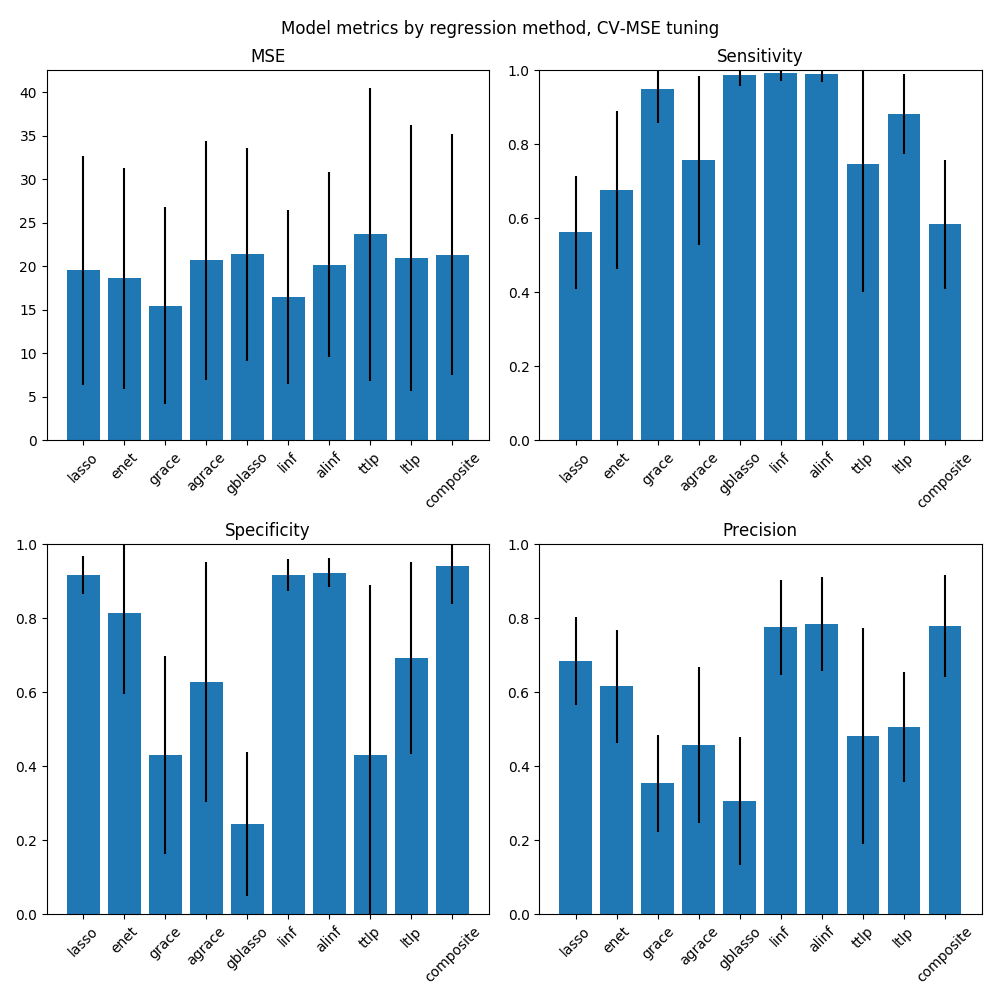
\includegraphics[scale=0.60]{cv_mse_tuning}
	\caption{CV-MSE tuning mean model metrics with standard deviation error bars for 20 synthetic datasets}
	\label{fig:met_cvmse}
\end{figure}

\section{Orchestrated tuning}
Subset of methods

\begin{table}[h!]
	\begin{center}
		\caption{Orchestrated tuning model metrics by regression method}
		\label{tab:met_orctun}
		\pgfplotstabletypeset[
		multicolumn names,
		col sep=comma,
		header=has colnames,
		columns={Method,MSE,Correlation,Sensitivity,Specificity,Precision},
		display columns/0/.style={string type, column type = {l}},
		display columns/1/.style={column type={S}, string type, column type = {c}},
		display columns/2/.style={column name=Correlation, column type={S}, string type, column type = {c}},
		display columns/3/.style={column name=Sensitivity, column type={S}, string type, column type = {c}},
		display columns/4/.style={column name=Specificity, column type={S}, string type, column type = {c}},
		display columns/5/.style={column name=Precision, column type={S}, string type, column type = {c}},
		every head row/.style={
			before row={\toprule}, 
			after row/.add={}{
				\arraybackslash
				&$(\sigma_{MSE})$&$(\sigma_{Correlation})$&($\sigma_{Sensitivity})$&$(\sigma_{Specificity})$&$(\sigma_{Precision})$\\
				\midrule\midrule
			}
		},
		every last row/.style={
			after row=\bottomrule
		},
		every nth row={2}{before row=\midrule},
		]{tables/metrics_orctun.csv}
	\end{center}
\end{table}
\begin{figure}[H]
	\centering
	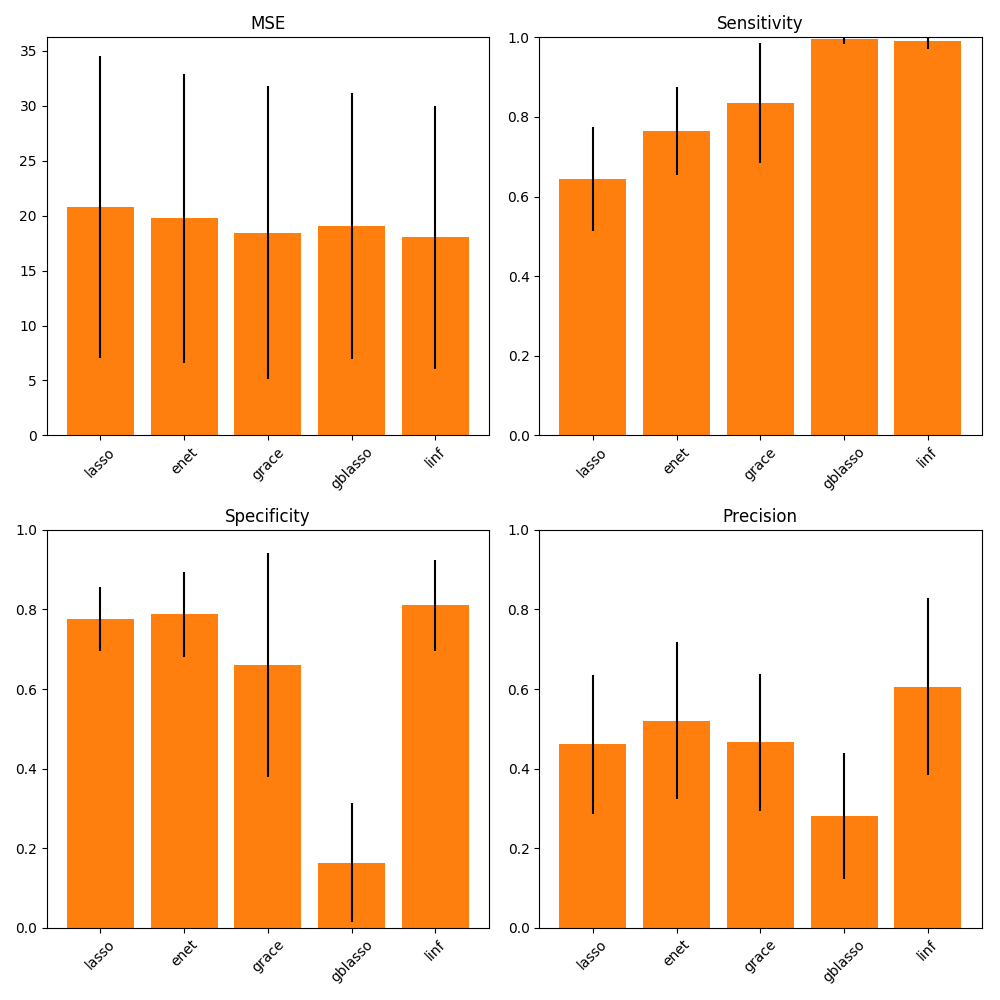
\includegraphics[scale=0.60]{orchestrated_tuning}
	\caption{Orchestrated tuning mean model metrics with standard deviation error bars for 20 synthetic datasets}
	\label{fig:met_orchestrated}
\end{figure}

\section{Comparison of tuning approaches}
\begin{table}[H]
	\begin{center}
		\caption{Comparison of mean model metrics by parameter tuning method}
		\label{tab:met_comp}
		\pgfplotstabletypeset[
		multicolumn names,
		col sep=comma,
		header=has colnames,
		columns={Method,Tuning,MSE,Correlation,Sensitivity,Specificity,Precision},
		display columns/0/.style={string type, column type = {l}},
		display columns/1/.style={string type, column type = {l}},
		display columns/2/.style={column type={S}, string type, column type = {r}},
		display columns/3/.style={column name=Correlation, column type={S}, string type, column type = {r}},
		display columns/4/.style={column name=Sens, column type={S}, string type, column type = {r}},
		display columns/5/.style={column name=Spec, column type={S}, string type, column type = {r}},
		display columns/6/.style={column name=Prec, column type={S}, string type, column type = {r}},
		every head row/.style={
			before row={\toprule}, 
			after row={\midrule\midrule}
		},
		every last row/.style={
			after row=\bottomrule
		},
		every nth row={2}{before row=\midrule},
		]{tables/metrics_comparison.csv}
	\end{center}
\end{table}
\begin{figure}[H]
	\centering
	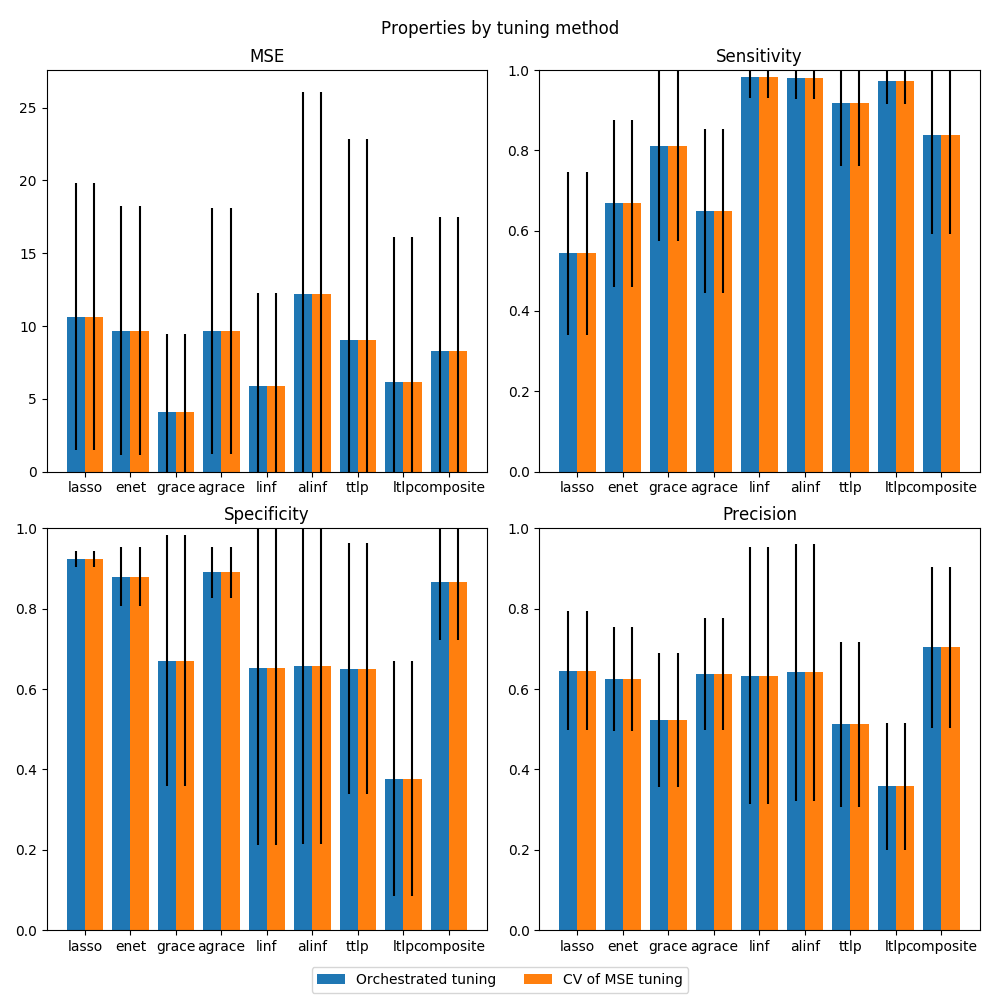
\includegraphics[scale=0.60]{tuning_method_comparison}
	\caption{Comparison of mean model metrics by parameter tuning method}
	\label{fig:met_comparison}
\end{figure}

\section{Optimal hyperparameter value selection}

\subsubsection{Lasso}
\begin{figure}[H]
	\centering
	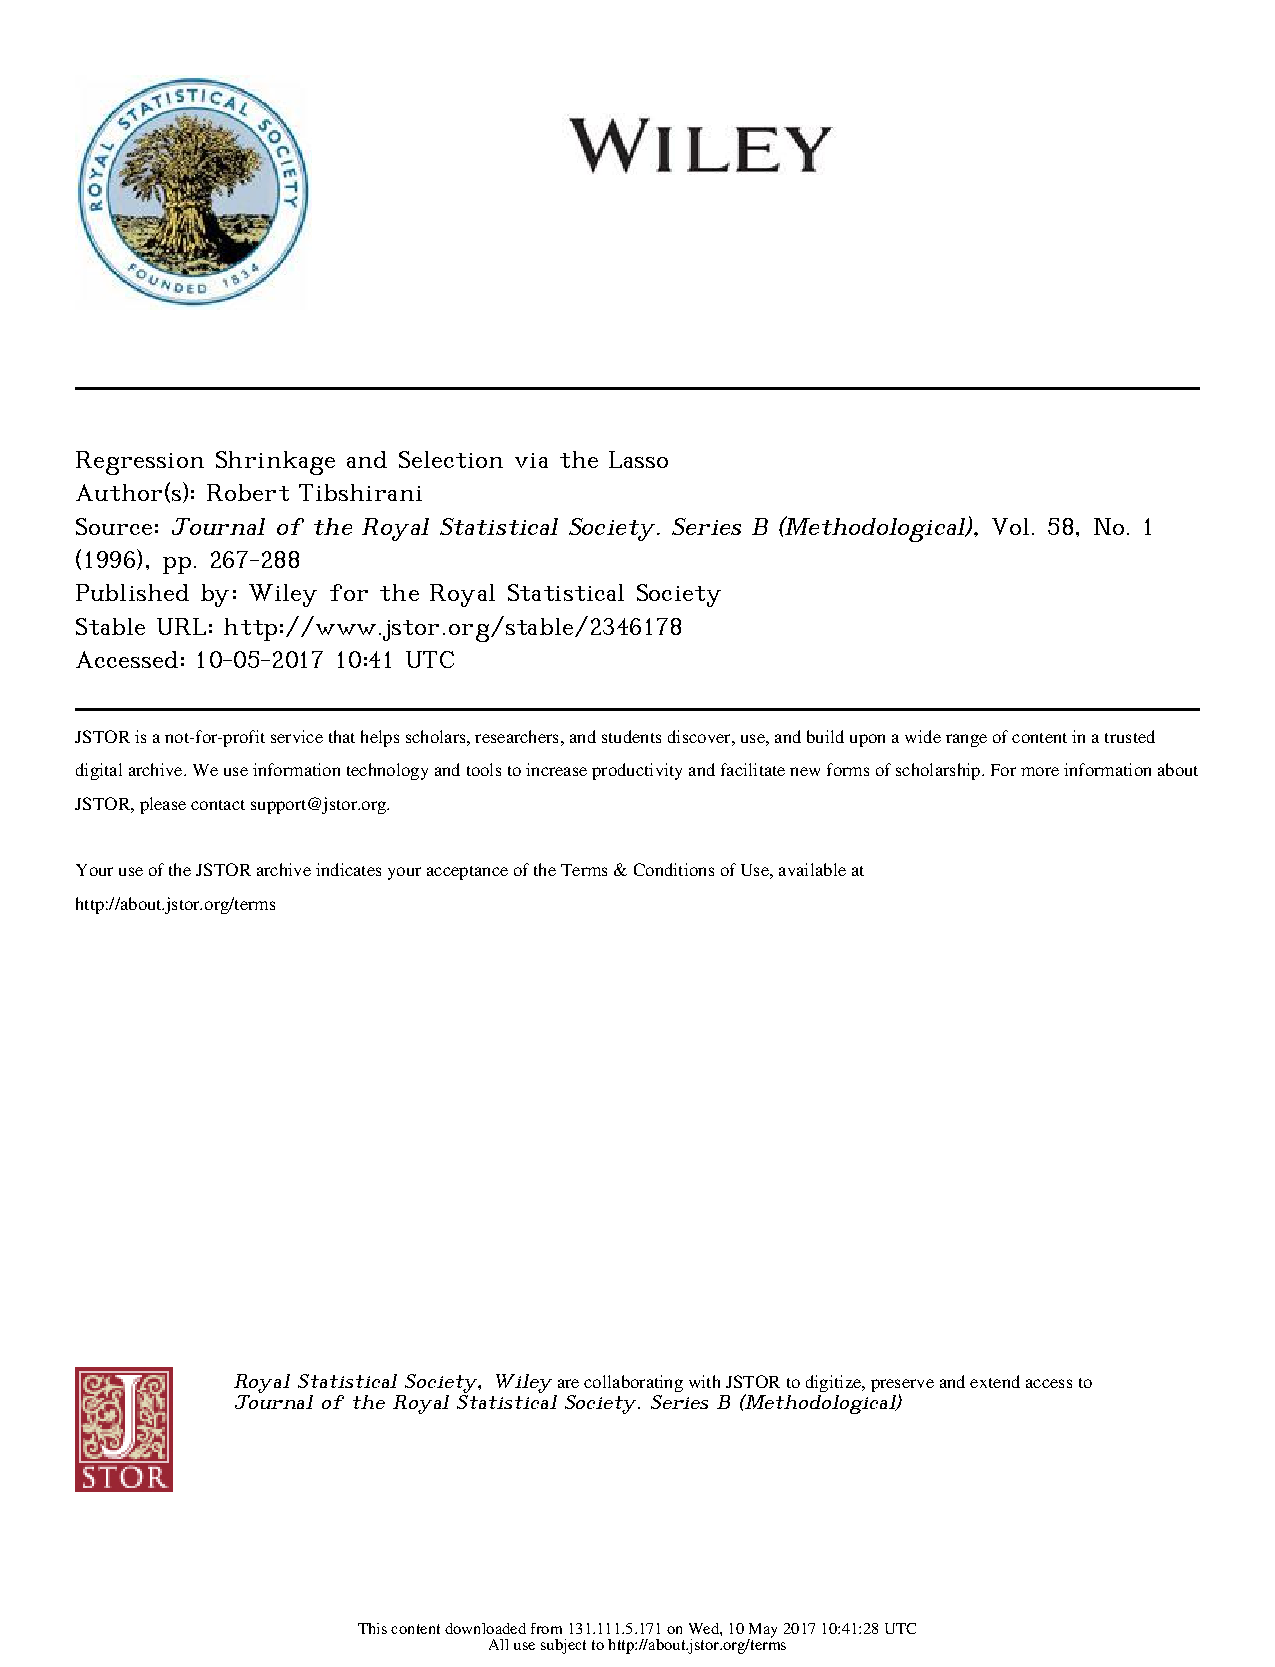
\includegraphics[scale=0.70]{tuning/lasso}
	\caption{Lasso method distribution of optimal tuning parameters}
	\label{fig:tun_lasso}
\end{figure}

\subsubsection{Elastic Net}
\begin{figure}[H]
	\centering
	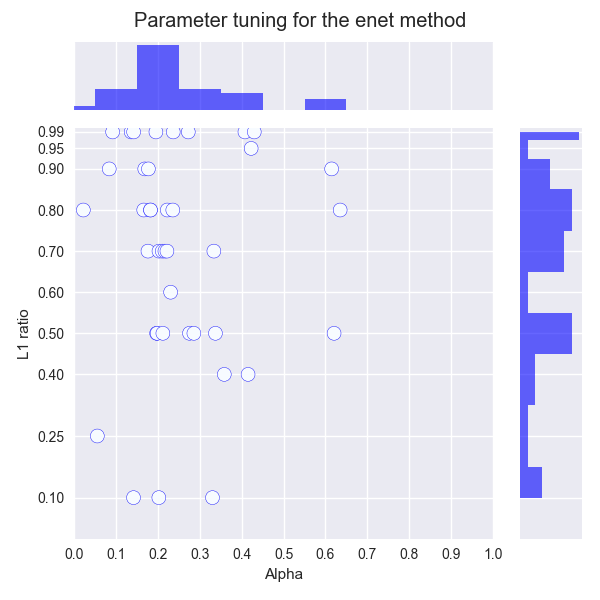
\includegraphics[scale=0.80]{tuning/enet}
	\caption{Elastic Net method distribution of optimal tuning parameters}
	\label{fig:tun_enet}
\end{figure}

\subsubsection{Grace}
\begin{figure}[H]
	\centering
	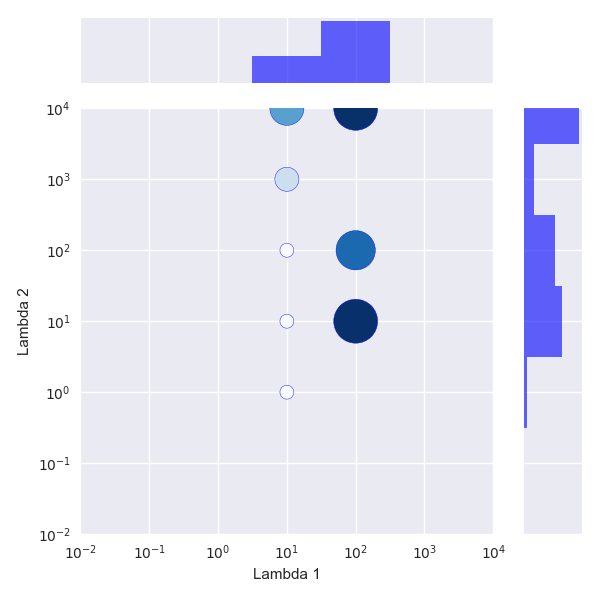
\includegraphics[scale=0.80]{tuning/grace}
	\caption{Grace method distribution of optimal tuning parameters}
	\label{fig:tun_grace}
\end{figure}

\subsubsection{aGrace}
\begin{figure}[H]
	\centering
	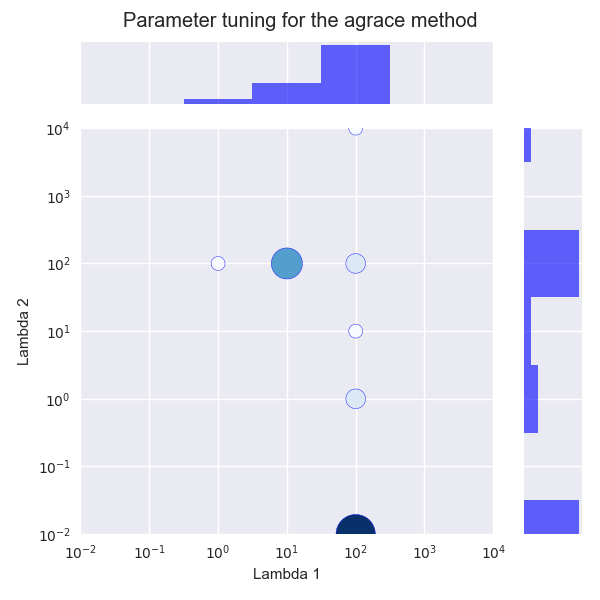
\includegraphics[scale=0.80]{tuning/agrace}
	\caption{aGrace method distribution of optimal tuning parameters}
	\label{fig:tun_agrace}
\end{figure}

\subsubsection{GBLasso}
\begin{figure}[H]
	\centering
	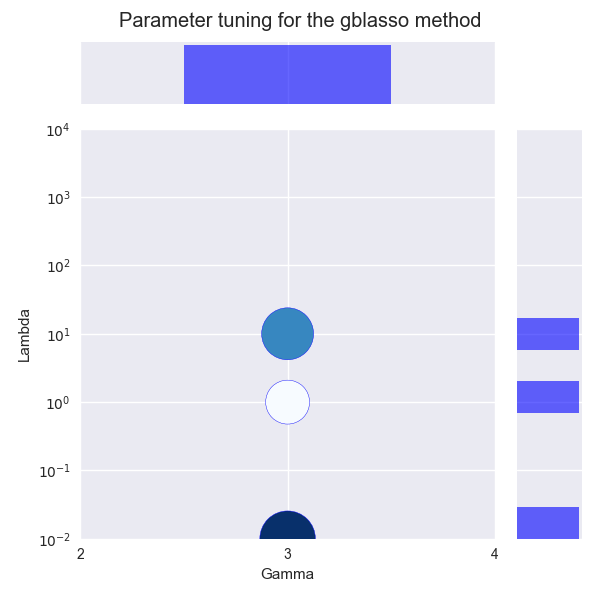
\includegraphics[scale=0.80]{tuning/gblasso}
	\caption{GBLasso method distribution of optimal tuning parameters}
	\label{fig:tun_gblasso}
\end{figure}

\subsubsection{Linf}
\begin{figure}[H]
	\centering
	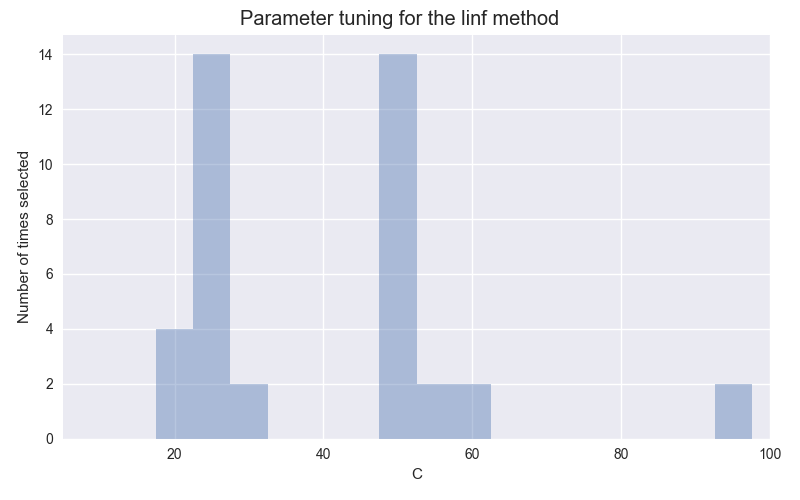
\includegraphics[scale=0.70]{tuning/linf}
	\caption{Linf method distribution of optimal tuning parameters}
	\label{fig:tun_linf}
\end{figure}

\subsubsection{aLinf}
\begin{figure}[H]
	\centering
	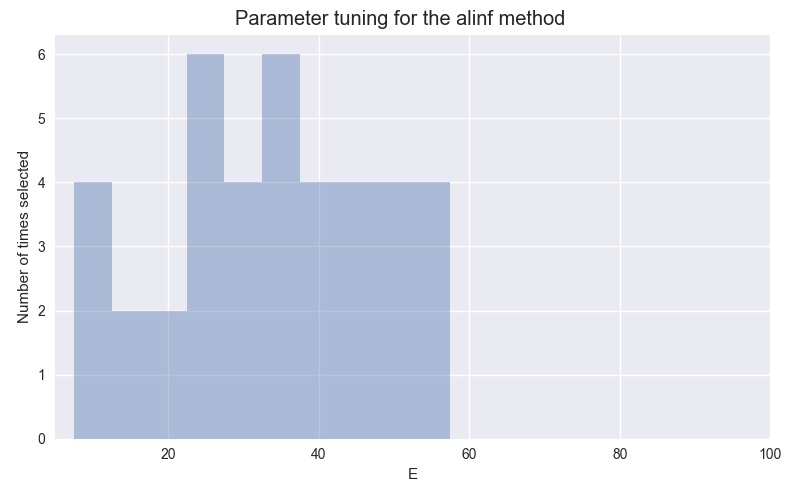
\includegraphics[scale=0.70]{tuning/alinf}
	\caption{aLinf method distribution of optimal tuning parameters}
	\label{fig:tun_alinf}
\end{figure}

\subsubsection{TTLP and LTLP}
The TTLP and LTLP methods use search spaces for their tuning parameters derived from dataset properties and the Lasso estimate. For this reason attempting to extract an optimal combination of hyperparameter values from tuning with external independent datasets is not feasible. 

\subsubsection{Composite}
\begin{figure}[H]
	\centering
	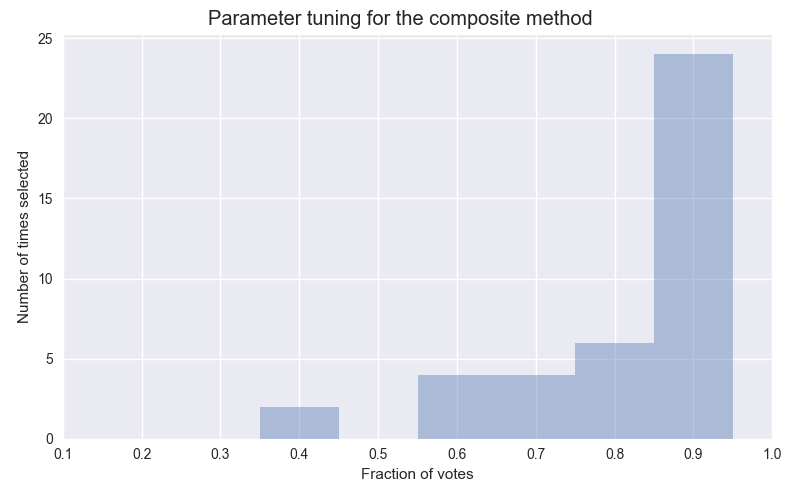
\includegraphics[scale=0.70]{tuning/composite}
	\caption{Composite method distribution of optimal tuning parameters}
	\label{fig:tun_composite}
\end{figure}
